\documentclass{article}

\usepackage{/home/paul/Workspace/build/macros}


\title{Examen 2025: corrigé}
\date{}
\author{Paul Catala}


\begin{document}
\maketitle

\section{Question de cours}

\begin{enumerate}
	\item La courbe bleue est celle qui converge le plus rapidement: il s'agit de la solution avec pas optimal. La courbe rouge est celle qui converge le moins rapidement: il s'agit de la solution avec pas constant. La courbe verte restante est la solution avec backtracking.
	
	\item 
	\begin{enumerate}
		\item Cette décomposition n'est pas une SVD car la matrice $U$ n'est pas orthogonale: en effet, 
		\eq{
			\begin{bmatrix}\frac{1}{\sqrt{2}} & \frac{1}{\sqrt{2}} \\ 0 & 1 \end{bmatrix}\begin{bmatrix}\frac{1}{\sqrt{2}} & 0 \\ \frac{1}{\sqrt{2}} & 1 \end{bmatrix}  = \begin{bmatrix} 1 & \frac{1}{\sqrt{2}} \\ \frac{1}{\sqrt{2}} & 1 \end{bmatrix} \neq I_2
		}
		
		\item Cette décomposition est une SVD: on vérifie bien que $U$ et $V$ sont orthogonales, et que $S$ est diagonale avec entrées positives.
		
		\item Cette décomposition n'est pas une SVD car les entrées diagonales de $S$ ne sont pas toutes positives
		
		\item Cette décomposition n'est pas une SVD car ni $U$ ni $V$ ne sont orthogonales.
	\end{enumerate}
		
	\item 
	\begin{enumerate}
		\item On a $z_1 = w_{11}x_1 + w_{12}x_2 = w_{13}x_3 + b_1 = \mathbf{w}_1^\top \mathbf{x} + b_1$, et de même $y_2 = \mathbf{w}_2^\top \mathbf{x} + b_2$.
		\item On a $y = v_1 \sigma(z_1) + v_2 \sigma(z_2) = v_1 \sigma(\mathbf{w}_1^\top \mathbf{x}) + v_2 \sigma(\mathbf{w}_2^\top \mathbf{x})$.
	\end{enumerate}
\end{enumerate}
	



\section{Optimisation numérique}

\begin{enumerate}
	\item Ce problème admet un minimiseur, car le critère est une fonction convexe de $\mathbf{R}^3$. L'unicité du minimiseur dépend des propriétés de $A$: ici, la matrice $A$ est de rang $2$, et a donc un noyau non réduit à $\{0\}$. Autrement dit, si $x_0$ est une solution du problème, alors pour tout $\mathbf{z} \in \Ker A$, $\mathbf{x}_0 + \mathbf{z}$ est aussi solution (car $\mathbf{A}(\mathbf{x}_0 + \mathbf{z}) = \mathbf{A}\mathbf{x}_0$).
	
	\item On a 
	\eq{
		\begin{aligned}
		f(\mathbf{x}) 
			&= \frac{1}{2}(\mathbf{A}\mathbf{x}-\mathbf{y})^\top (\mathbf{A}\mathbf{x}-\mathbf{y}) +\frac{1}{2} \mathbf{x}^\top\mathbf{x}\\
			&= \frac{1}{2}\mathbf{x}^\top \mathbf{A}^\top \mathbf{A}\mathbf{x} - \frac{1}{2}\mathbf{x}^\top\mathbf{A}^\top \mathbf{y} - \frac{1}{2}\mathbf{y}^\top \mathbf{A}\mathbf{x} + \frac{1}{2}\mathbf{y}^\top \mathbf{y} + \frac{1}{2}\mathbf{x}^\top \mathbf{x}\\
			&= \frac{1}{2}\mathbf{x}^\top(\mathbf{A}^\top\mathbf{A} + \mathbf{I})\mathbf{x} - (\mathbf{A}^\top \mathbf{y})^\top \mathbf{x} + \frac{1}{2}\norm{\mathbf{y}}^2\\
			&= \frac{1}{2}\mathbf{x}^\top \mathbf{P}\mathbf{x} + \mathbf{q}^\top \mathbf{x} + r.
		\end{aligned}
	}
	où $\mathbf{P} = \mathbf{A}^\top \mathbf{A} + \mathbf{I}$, $\mathbf{q} = -\mathbf{A}^\top \mathbf{y}$ et $r = 1/2\norm{\mathbf{y}}^2$.
	
	\item On a
	\eq{
		\begin{aligned}
			&\frac{\partial}{\partial \mathbf{x}} \left( \frac{1}{2}\mathbf{x}^\top\mathbf{P}\mathbf{x} \right) = \mathbf{P}\mathbf{x}\\
			&\frac{\partial}{\partial \mathbf{x}} (\mathbf{q}^\top \mathbf{x}) = \mathbf{q}\\
			&\frac{\partial}{\partial \mathbf{x}} r = 0.
		\end{aligned}
	}
	Par conséquent, le gradient de $f$ en $\mathbf{x}$ est donné par
	\eq{
		\nabla f(\mathbf{x}) = \mathbf{P}\mathbf{x} + \mathbf{q} = (\mathbf{A}^\top \mathbf{A} + \mathbf{I})\mathbf{x} - \mathbf{A}^\top \mathbf{y}.
	}
	
	\item La fonction $f$ est convexe, donc tout minimiseur local est un minimiseur global. Une condition nécessaire et suffisante d'optimalité est donc 
	\eq{
		\nabla f(\mathbf{x}_*) = 0
	}
	On en déduit
	\eq{
		(\mathbf{A}^\top \mathbf{A} + \mathbf{I})\mathbf{x}_* = \mathbf{A}^\top \mathbf{y}.
	}
	Or
	\eq{
		\mathbf{A}^\top \mathbf{A} + \mathbf{I} = \begin{bmatrix} 4 & -3 & 0 \\ -3 & 4 & 0 \\ 0 & 0 & 7\end{bmatrix}
	}
	est inversible (déterminant non nul). On obtient donc
	\eq{
		\mathbf{x}_* = (\mathbf{A}^\top \mathbf{A} + \mathbf{I})^{-1} \mathbf{A}^\top \mathbf{y}.
	}
\end{enumerate} 

\section{Classification}

\subsection{Séparateur linéaire}

\begin{enumerate}
	\item 
		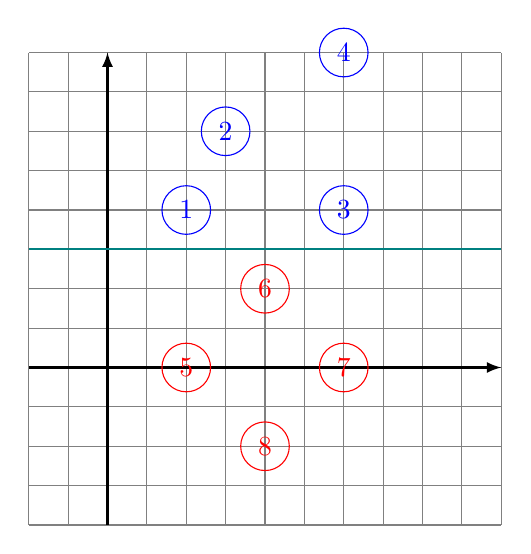
\begin{tikzpicture}
		
		\draw[gray] (-1,-2) -- (5,-2);
		\draw[gray] (-1,-1.5) -- (5,-1.5);
		\draw[gray] (-1,-1) -- (5,-1);
		\draw[gray] (-1,-0.5) -- (5,-0.5);
		\draw[gray] (-1,0) -- (5,0);
		\draw[gray] (-1,0.5) -- (5,0.5);
		\draw[gray] (-1,1) -- (5,1);
		\draw[gray] (-1,1.5) -- (5,1.5);
		\draw[gray] (-1,2) -- (5,2);
		\draw[gray] (-1,2.5) -- (5,2.5);
		\draw[gray] (-1,3) -- (5,3);
		\draw[gray] (-1,3.5) -- (5,3.5);
		\draw[gray] (-1,4) -- (5,4);
		
		\draw[gray] (-1,-2) -- (-1,4);
		\draw[gray] (-0.5,-2) -- (-0.5,4);
		\draw[gray] (0,-2) -- (0,4);
		\draw[gray] (0.5,-2) -- (0.5,4);
		\draw[gray] (1,-2) -- (1,4);
		\draw[gray] (1.5,-2) -- (1.5,4);
		\draw[gray] (2,-2) -- (2,4);
		\draw[gray] (2.5,-2) -- (2.5,4);
		\draw[gray] (3,-2) -- (3,4);
		\draw[gray] (3.5,-2) -- (3.5,4);
		\draw[gray] (4,-2) -- (4,4);
		\draw[gray] (4.5,-2) -- (4.5,4);
		\draw[gray] (5,-2) -- (5,4);
		
		\draw[-latex,thick] (-1,0) -- (5,0);
		\draw[-latex,thick] (0,-2) -- (0,4);
		
		\node[circle,blue,draw] at (1,2) {1};
		\node[circle,blue,draw] at (1.5,3) {2};
		\node[circle,blue,draw] at (3,2) {3};
		\node[circle,blue,draw] at (3,4) {4};
		
		\node[circle,red,draw] at (1,0) {5};
		\node[circle,red,draw] at (2,1) {6};
		\node[circle,red,draw] at (3,0) {7};
		\node[circle,red,draw] at (2,-1) {8};
		
		\draw[teal,thick] (-1,1.5) -- (5,1.5);
	\end{tikzpicture}
	
	\item L'hyperplan optimal est la droite horizontale d'équation $y = 3/2$. La marge est $2\times 0.5 = 1$.
	
	\item Les vecteurs de support sont les données $1,3$ pour la classe $+1$, et $6$ pour la classe $-1$.
	
	\subsection{Astuce du noyau}
	
	\item 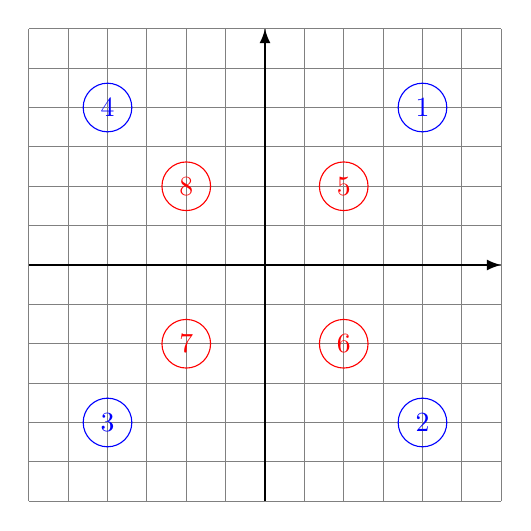
\begin{tikzpicture}
		
		\draw[gray] (-3,-3) -- (3,-3);
		\draw[gray] (-3,-2.5) -- (3,-2.5);
		\draw[gray] (-3,-2) -- (3,-2);
		\draw[gray] (-3,-1.5) -- (3,-1.5);
		\draw[gray] (-3,-1) -- (3,-1);
		\draw[gray] (-3,-0.5) -- (3,-0.5);
		\draw[gray] (-3,0) -- (3,0);
		\draw[gray] (-3,0.5) -- (3,0.5);
		\draw[gray] (-3,1) -- (3,1);
		\draw[gray] (-3,1.5) -- (3,1.5);
		\draw[gray] (-3,2) -- (3,2);
		\draw[gray] (-3,2.5) -- (3,2.5);
		\draw[gray] (-3,3) -- (3,3);
		
		\draw[gray] (-3,-3) -- (-3,3);
		\draw[gray] (-2.5,-3) -- (-2.5,3);
		\draw[gray] (-2,-3) -- (-2,3);
		\draw[gray] (-1.5,-3) -- (-1.5,3);
		\draw[gray] (-1,-3) -- (-1,3);
		\draw[gray] (-0.5,-3) -- (-0.5,3);
		\draw[gray] (0,-3) -- (0,3);
		\draw[gray] (0.5,-3) -- (0.5,3);
		\draw[gray] (1,-3) -- (1,3);
		\draw[gray] (1.5,-3) -- (1.5,3);
		\draw[gray] (2,-3) -- (2,3);
		\draw[gray] (2.5,-3) -- (2.5,3);
		\draw[gray] (3,-3) -- (3,3);
		
		\draw[-latex,thick] (-3,0) -- (3,0);
		\draw[-latex,thick] (0,-3) -- (0,3);
		
		\node[circle,blue,draw] at (2,2) {1};
		\node[circle,blue,draw] at (2,-2) {2};
		\node[circle,blue,draw] at (-2,-2) {3};
		\node[circle,blue,draw] at (-2,2) {4};
		
		\node[circle,red,draw] at (1,1) {5};
		\node[circle,red,draw] at (1,-1) {6};
		\node[circle,red,draw] at (-1,-1) {7};
		\node[circle,red,draw] at (-1,1) {8};
		
	\end{tikzpicture}
	
	Les deux classes ne sont pas linéairement séparables.
	
	\item L'astuce du noyau consiste à appliquer une transformation aux données, de manière à les rendre linéairement séparables dans le nouvel espace de représentation.
	
	\item Les données de la classe négative sont inchangées par cette transformation, car elles sont toutes de norme inférieure à 2. Les nouvelles coordonnées des points de la classe positive sont
	\eq{
		(3,3), (11,7), (7,7), (11,7)
	}
	Les classes sont linéairement séparables dans cet espace de représentation.
	
	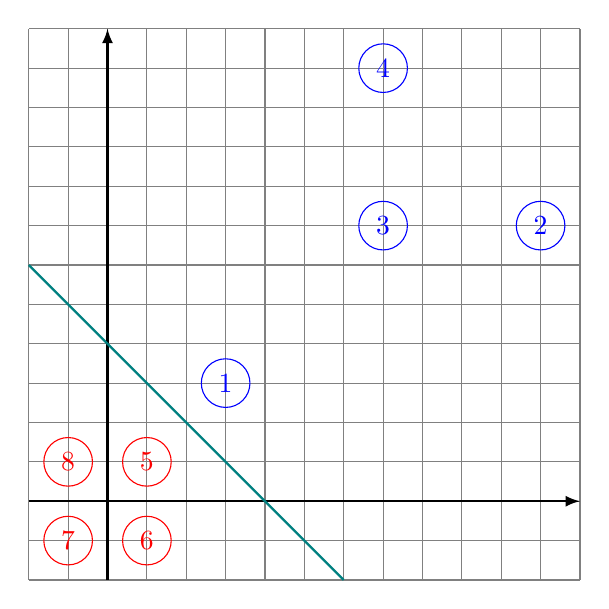
\begin{tikzpicture}

	\draw[step=0.5,gray] (-1,-1) grid (6,6);

	\draw[-latex,thick] (-1,0) -- (6,0);
	\draw[-latex,thick] (0,-1) -- (0,6);
	
	\node[circle,blue,draw] at (1.5,1.5) {1};
	\node[circle,blue,draw] at (5.5,3.5) {2};
	\node[circle,blue,draw] at (3.5,3.5) {3};
	\node[circle,blue,draw] at (3.5,5.5) {4};
	
	
	\node[circle,red,draw] at (0.5,0.5) {5};
	\node[circle,red,draw] at (0.5,-0.5) {6};
	\node[circle,red,draw] at (-0.5,-0.5) {7};
	\node[circle,red,draw] at (-0.5,0.5) {8};
	
	\draw[teal,thick] (-1,3) -- (3,-1);

	\end{tikzpicture}
	
	\item L'hyperplan optimal est la droite d'équation $y = -x + 4$. La marge est $2\times \sqrt{2} = 2\sqrt{2}$.
	
	\item Si l'on applique la transformation à l'échantillon $(6,6)$, on obtient comme nouvelles coordonnées $(-1,-1)$. Avec ce noyau, l'échantillon sera donc (probablement faussement) classé négatif.
	
	\item Une transformation possible est $\psi : (x_1,x_2) \mapsto (x_1,x_2,x_1^2+x_2^2)$, pour séparer les données selon leur norme euclidienne.
	
	
	\end{enumerate}
	
	
	\section{Décompositions matricielles}
	
	\begin{enumerate}
		\item 
		\begin{enumerate}
			\item On a
			\eq{
				\mathbf{B} = \begin{bmatrix} 3 & -3 & 0 \\ -3 & 3 & 0 \\ 0 & 0 & 6\end{bmatrix}
			}
			
			\item $\mathbf{B}$ est de rang $2$ (les deux premières colonnes sont colinéaires). $\mathbf{B}$ a donc un noyau non réduit à $0$, ce qui signifie qu'il existe $\mathbf{x}$ tel que $\mathbf{B}\mathbf{x} = 0 = 0 \cdot\mathbf{x}$. $0$ est donc une valeur propre de $\mathbf{B}$. Un vecteur du noyau est donné par
			\eq{
				\mathbf{v}_0 = \begin{bmatrix} 1 \\ 1 \\ 0 \end{bmatrix}
			}
			
			\item On a
			\eq{
				\mathbf{B} - 6\mathbf{I}_3 = \begin{bmatrix} -3 & -3 & 0 \\ -3 & -3 & 0 \\ 0 & 0 & 0 \end{bmatrix}
			}
			Cette matrice est de rang $1$.
			On a
			\eq{
				(\mathbf{B}-6\mathbf{I}_3) \begin{bmatrix} 1 \\ -1 \\ 0 \end{bmatrix} = \begin{bmatrix} 0 \\ 0 \\ 0 \end{bmatrix}, \quad \text{donc} \quad \mathbf{B} \begin{bmatrix} 1 \\ -1 \\ 0 \end{bmatrix} = 6 \cdot\begin{bmatrix} 1 \\ -1 \\ 0 \end{bmatrix}
			}
			et de même
			\eq{
				\mathbf{B} \begin{bmatrix} 0 \\ 0 \\ 1 \end{bmatrix} = 6 \cdot\begin{bmatrix} 0 \\ 0 \\ 1 \end{bmatrix}
			} 
			
			$\displaystyle \mathbf{v}_1 = \begin{bmatrix} 1\\-1\\0 \end{bmatrix}$ et $\displaystyle \mathbf{v}_2 = \begin{bmatrix} 0 \\ 0 \\ 1 \end{bmatrix}$ sont donc deux vecteurs propres non colinéaires associés à la valeur propre $6$.
			
			\item Les valeurs singulières de $A$ sont les racines des valeurs singulières de $\mathbf{B}$, c'est-à-dire $\sigma_1 = \sigma_2 = \sqrt{6}$ et $\sigma_3 = 0$. Les vecteurs singuliers droits associés sont $\mathbf{v}_1, \mathbf{v}_2$ et $\mathbf{v}_0$ respectivement (que l'on normalise usuellement).
		\end{enumerate}
		
		\item On a
		\eq{
			\begin{aligned}
				\Tr(\mathbf{X}^\top \mathbf{X}) 
					&= \Tr(\mathbf{V}\mathbf{\Sigma}\mathbf{U}^\top \mathbf{U}\mathbf{\Sigma}\mathbf{V^\top})\\
					&= \Tr(\mathbf{V}\mathbf{\Sigma}\mathbf{\Sigma}\mathbf{V^\top})\\
					&= \Tr(\mathbf{V^\top}\mathbf{V}\mathbf{\Sigma}^2)\\
					&= \Tr(\mathbf{\Sigma}^2)\\
					&= \sum_{i=1}^r \sigma_i^2
			\end{aligned}
		}
		où l'on a utilisé dans l'odre l'orthogonalité de $\mathbf{U}$, $\Tr(AB) = \Tr(BA)$, et l'orthogonlité de $\mathbf{V}$. Le résultat attendu s'obtient en élevant à la puissance $1/2$ l'équation précédente.
	
\end{enumerate}
	

\end{document}